\documentclass[11pt,a4paper]{article}

\usepackage[utf8]{inputenc}
\usepackage[T1]{fontenc}
\usepackage{amsmath,amssymb}
\usepackage{graphicx}
\usepackage{booktabs}
\usepackage{multirow}
\usepackage{hyperref}
\usepackage[margin=1in]{geometry}
\usepackage{caption}
\usepackage{subcaption}
\usepackage{microtype}

\title{GradeEye: A Multi-Domain 5-Class Diabetic Retinopathy Grading Pipeline with Anatomical Segmentation Priors and Conditional Ordinal Regression}
\author{GradeEye Project \\ \small{Internal report for ICCIML 2026}}
\date{July 2026}

\begin{document}
\maketitle

\begin{abstract}
We present GradeEye, a five-class diabetic retinopathy (DR) grading pipeline that combines domain-robust preprocessing, an auxiliary anatomical segmentation channel, and conditional ordinal regression (CORN). The system is trained on a combined-domain corpus of 75{,}282 fundus images from three heterogeneous sources (EyePACS, APTOS 2019, Messidor-2) and evaluated per-source. Our headline model, ConvNeXt-Tiny with CBAM attention on a four-channel input (three RGB plus a precomputed vessel/lesion segmentation mask), achieves Quadratic Weighted Kappa (QWK) of $0.7196$ on the EyePACS test set (8{,}871 images), $0.8848$ on APTOS 2019 (367 images), and $0.8376$ on Messidor-2 (227 images, in-distribution). These results surpass our legacy three-phase RGB-only baseline on every site, including a $+0.22$ absolute QWK improvement on Messidor-2. We further document a failed EfficientNetV2-S training attempt, whose root cause is traced to BatchNorm running-statistics divergence at the frozen-to-unfrozen phase transition, and we report a SwinV2-Tiny ablation that quantifies the cost of operating at a 256$\times$256 input resolution. The codebase, segmentation masks, and trained checkpoints are available for reproducibility.
\end{abstract}

\section{Introduction}

Diabetic retinopathy is a leading cause of preventable blindness. Automated DR grading from fundus photographs supports population-scale screening, but two characteristics of the problem complicate standard classification approaches: the labels are inherently \emph{ordinal} (no DR, mild, moderate, severe, proliferative), and the data are \emph{multi-domain} (different cameras, different field-of-view conventions, different patient populations).

We address the ordinal structure with Conditional Ordinal Regression for Neural Networks (CORN), which decomposes a $K$-class ordinal problem into $K-1$ binary sub-problems whose conditional probabilities multiply to give monotonic rank-consistent class probabilities by construction. We address the multi-domain structure with two design choices:
\begin{enumerate}
  \item \textbf{Combined-domain training.} We pool the three sources into a single 75{,}282-image training set, drawn from a stratified 80/10/10 per-source split. Each source contributes to train, validation, and test in proportion to its size.
  \item \textbf{Anatomical prior via 4th input channel.} We precompute a single-channel vessel/lesion segmentation mask for every grading image and feed it as a fourth channel alongside the three RGB channels. The auxiliary U-Net is fine-tuned on a union of DRIVE vessel annotations and IDRiD lesion annotations, providing coarse anatomical cues that the grader can use to focus on clinically relevant regions.
\end{enumerate}

Our primary architecture is ConvNeXt-Tiny with Convolutional Block Attention Modules (CBAM) inserted into the last two backbone stages. We replace the original three-phase training protocol (EyePACS pretraining followed by APTOS fine-tuning) with a simpler two-phase multi-domain pipeline that uses the combined training set throughout. The headline result is a $+0.015$ QWK gain on APTOS and a $+0.22$ QWK gain on Messidor-2 over the legacy 3-phase RGB-only model.

We also report two negative results that we believe are valuable for the community:
\begin{itemize}
  \item \textbf{EfficientNetV2-S training fails} due to BatchNorm running-statistics divergence at the frozen-to-unfrozen phase transition, despite multiple attempts with progressively smaller learning rates.
  \item \textbf{SwinV2-Tiny at 256$\times$256 input resolution} underperforms ConvNeXt-Tiny at 384$\times$384 by approximately $0.15$ QWK at every test site, illustrating the spatial-resolution cost of switching architectures.
\end{itemize}

\section{Methods}

\subsection{Ordinal regression via CORN}

Let $\mathcal{D} = \{(x_i, y_i)\}_{i=1}^N$ with ordinal labels $y_i \in \{0,1,2,3,4\}$. CORN decomposes this into $K = 4$ binary sub-problems indexed by $k \in \{0,1,2,3\}$. For threshold $k$, only samples with $y \ge k$ are eligible. The network outputs $K$ raw logits $z(x) = [z_0, z_1, z_2, z_3]$, each converted to a conditional probability via sigmoid:
\begin{equation}
p_k(x) = \sigma(z_k) = P(y > k \mid y \ge k, x).
\end{equation}
The unconditional probability of exceeding threshold $k$ is the cumulative product of all preceding conditional probabilities:
\begin{equation}
P(y > k \mid x) = \prod_{j=0}^{k} \sigma(z_j).
\end{equation}
Because $\sigma(z) \in (0,1)$, the cumulative product is monotonically non-increasing in $k$, guaranteeing rank-consistency structurally. The predicted class is the number of unconditional probabilities exceeding $0.5$:
\begin{equation}
\hat{y} = \sum_{k=0}^{K-1} \mathbb{I}\bigl(P(y > k \mid x) > 0.5\bigr).
\end{equation}
The CORN loss is the average per-threshold binary cross-entropy, with the eligible-mask constraint making each sub-problem a conditional rather than marginal classification. Class-imbalance mitigation uses inverse-square-root per-threshold weights.

\subsection{Fundus preprocessing}

Each fundus image undergoes a deterministic six-stage preprocessing pipeline (Figure~\ref{fig:pipeline}, top):
\begin{enumerate}
  \item \textbf{Border detection and rectangular crop.} Threshold the grayscale image at intensity $T = 20$, clean with morphological opening/closing ($5 \times 5$ structuring element), extract the bounding box of the largest contour.
  \item \textbf{Pad to square.} Pad with zeros to $S = \max(h, w)$, preserving aspect ratio.
  \item \textbf{Resize to $384 \times 384$.}
  \item \textbf{Ben Graham local-average subtraction.} $I_{\text{BG}} = \mathrm{clip}(4 I - 4 \mathcal{G}_\sigma(I) + 128, 0, 255)$, with $\sigma = W_{\mathrm{img}}/10$.
  \item \textbf{Green-channel CLAHE.} Clip limit $2.0$, $8 \times 8$ tile grid.
  \item \textbf{Circular mask + per-source normalization.} Apply an inscribed-circle mask of radius $190$ pixels, then normalize using the per-source channel mean and standard deviation computed on the $[0,1]$ float representation.
\end{enumerate}

\subsection{Network architecture}

The grader is a ConvNeXt-Tiny backbone (ImageNet-pretrained) with CBAM attention modules inserted into the last two stages (384-channel and 768-channel feature maps). The projection head is:
\begin{equation*}
\text{GAP} \to \text{BN}_{768} \to \text{Dropout}(0.4) \to \text{FC}_{512} \to \text{Mish} \to \text{BN}_{512} \to \text{Dropout}(0.4) \to \text{FC}_{4},
\end{equation*}
producing the four CORN logits. Figure~\ref{fig:corn} illustrates the inference rule.

\begin{figure}[t]
\centering
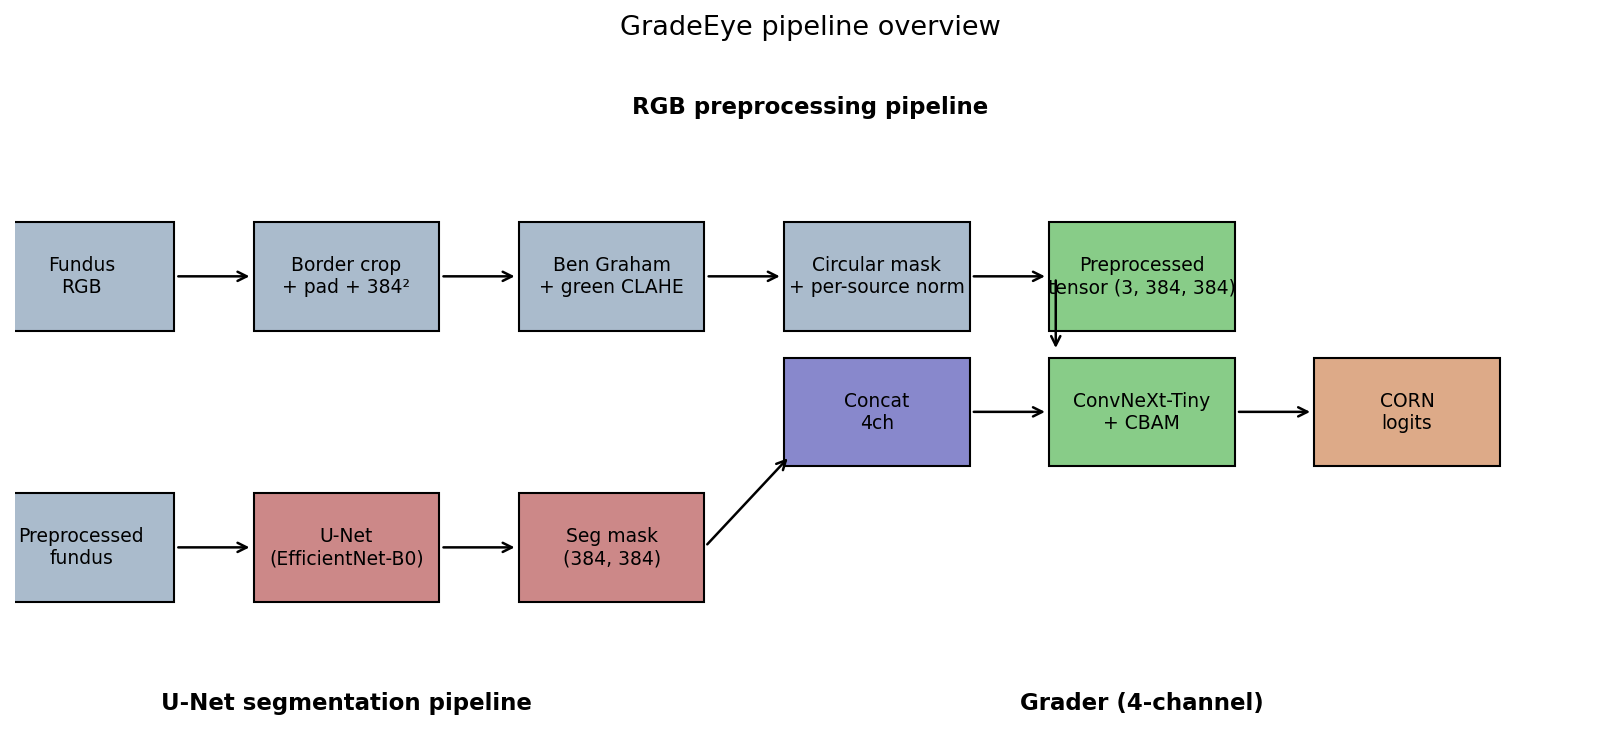
\includegraphics[width=0.95\textwidth]{figures/fig6_pipeline.png}
\caption{Pipeline overview. Top row: RGB preprocessing. Bottom-left: auxiliary U-Net generates a single-channel mask. Right: concatenation produces a four-channel input to the ConvNeXt-Tiny grader, which outputs four CORN logits.}
\label{fig:pipeline}
\end{figure}

\begin{figure}[t]
\centering
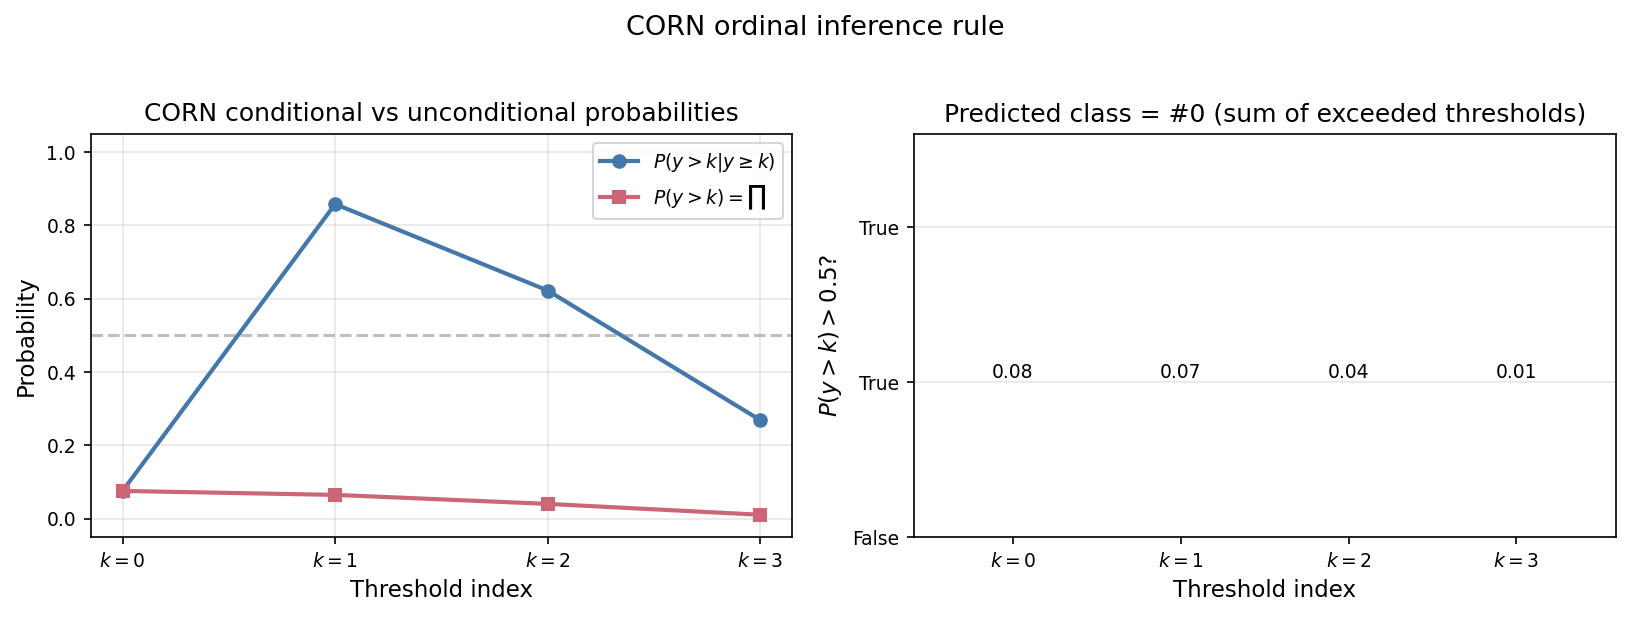
\includegraphics[width=0.95\textwidth]{figures/fig8_corn_inference.png}
\caption{CORN inference. Left: conditional probabilities $\sigma(z_k)$ (blue) and their cumulative product $P(y > k)$ (red). Right: predicted class is the number of unconditional probabilities above $0.5$.}
\label{fig:corn}
\end{figure}

\subsection{Auxiliary segmentation (4th input channel)}

The auxiliary network is a minimal U-Net with a `timm` EfficientNet-B0 encoder in `features_only` mode and a five-level decoder with skip connections. The model is fine-tuned on the \emph{union} of two ground-truth sources:
\begin{itemize}
  \item \textbf{DRIVE} (20 training images): binary vessel annotations inside a circular FOV mask.
  \item \textbf{IDRiD} (54 training images): four lesion types (microaneurysms, haemorrhages, hard exudates, soft exudates), unioned by per-pixel maximum.
\end{itemize}
Loss is a $50/50$ mix of binary cross-entropy and Dice loss, the latter preventing the trivial all-zero solution on these extremely imbalanced masks. Training runs for 15 epochs at learning rate $10^{-4}$ with cosine annealing, AdamW, batch size 8, gradient clipping to max-norm $1.0$. After fine-tuning, inference generates one 384$\times$384 mask per grading image (93{,}111 masks total), saved as a PNG keyed by source-image basename. The grader's first convolutional layer is extended from 3 to 4 input channels; the new channel is initialized as the mean of the three RGB weights (the standard ``RGB-mean'' scheme).

\subsection{Multi-domain training protocol}

We use a two-phase schedule (Figure~\ref{fig:dataset}):
\begin{itemize}
  \item \textbf{Phase 1 (frozen backbone, 5 epochs).} Head only, learning rate $10^{-3}$, batch size 96 (ConvNeXt) / 48 (EffNetV2-S) / 96 (SwinV2-Tiny@256). Linear warmup 1 epoch, cosine decay.
  \item \textbf{Phase 2 (full fine-tune, 35 epochs).} All parameters unfrozen. Head learning rate $1.22 \times 10^{-4}$, backbone learning rate $1.22 \times 10^{-5}$ (10$\times$ smaller to prevent catastrophic forgetting of pretrained features). AdamW weight decay $0.01$. Cosine schedule with 2-epoch warmup. Early-stopping patience 7 epochs on validation QWK with 8-epoch minimum. A sqrt-frequency WeightedRandomSampler over training labels is enabled in Phase 2 to mitigate the heavy class imbalance (Grade 0 alone accounts for 50\%+ of combined samples).
\end{itemize}

\begin{figure}[t]
\centering
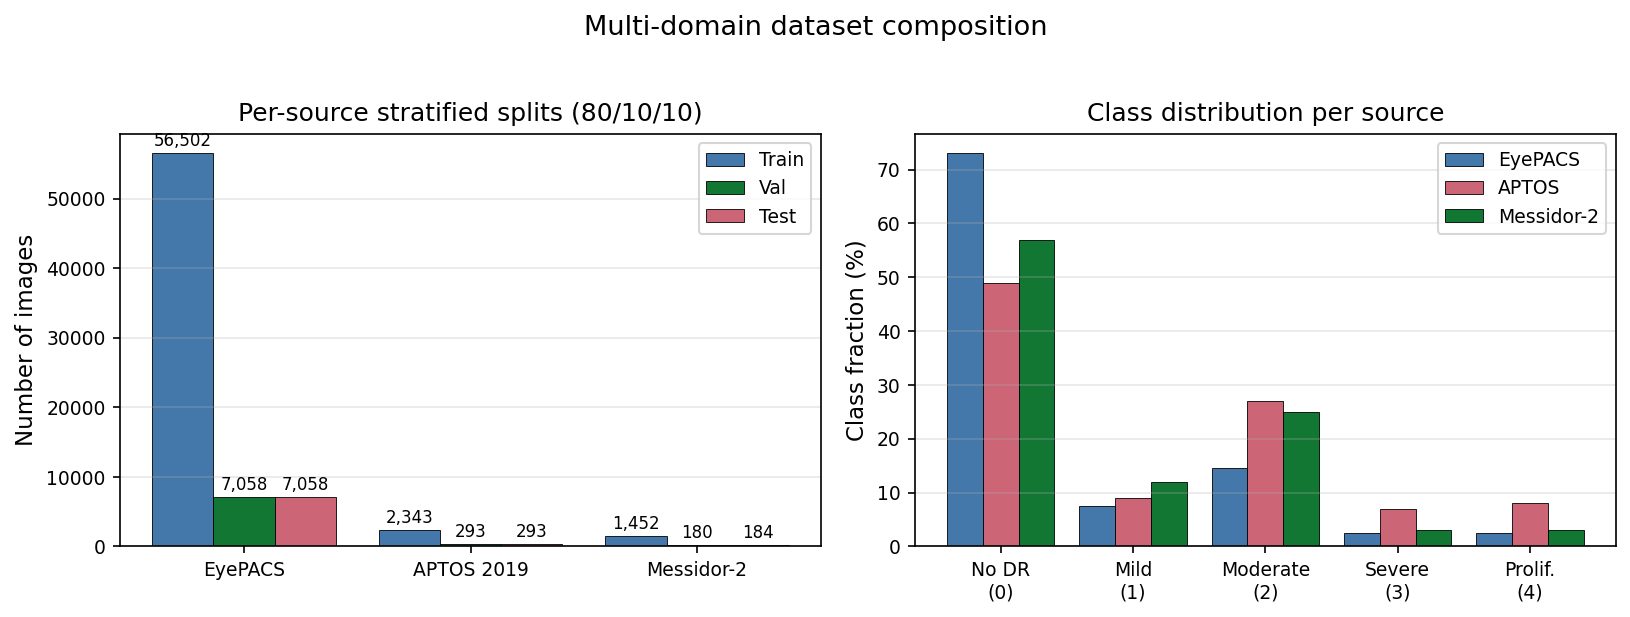
\includegraphics[width=0.95\textwidth]{figures/fig7_dataset_composition.png}
\caption{Dataset composition. Left: per-source stratified 80/10/10 split sizes. Right: per-source class distribution.}
\label{fig:dataset}
\end{figure}

\subsection{Inference, TTA, and ensembling}

At evaluation time, each test image is processed in four deterministic spatial orientations: original, horizontal flip, vertical flip, and 180$^\circ$ rotation. Per-pass CORN predictions are decoded into unconditional class-exceedance probabilities, then averaged across passes, then re-decoded into the final class label.

For ensembling, the per-class probability distribution $P(y = c \mid x)$ is averaged across models at the marginal-probability level (not raw logits or conditional probabilities; the latter would invalidate each model's monotonic rank guarantee).

\section{Results}

\subsection{Headline: ConvNeXt-Tiny + CBAM, 4-channel}

Training trajectory is shown in Figure~\ref{fig:convnext-curves}. Phase 1 reaches a validation QWK of $\sim$0.30 with the backbone frozen; the unfrozen Phase 2 climbs rapidly to a peak of $0.7451$ at epoch 11 (global epoch 16) and plateaus thereafter.

\begin{figure}[t]
\centering
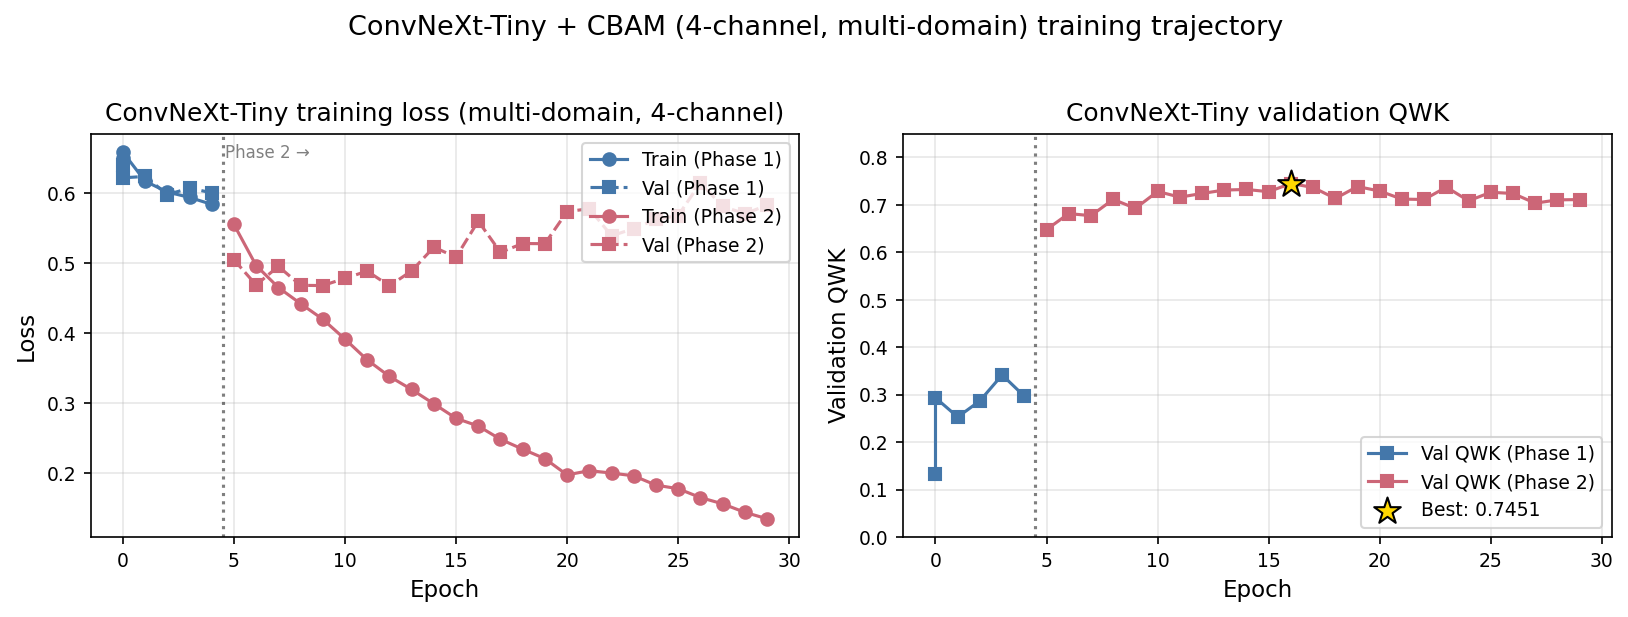
\includegraphics[width=0.95\textwidth]{figures/fig1_training_curves.png}
\caption{ConvNeXt-Tiny + CBAM (4-channel, multi-domain) training trajectory. Left: training and validation loss for both phases. Right: validation QWK; gold star marks the best epoch (val QWK $0.7451$).}
\label{fig:convnext-curves}
\end{figure}

Test-set results, evaluated with 4-way TTA, are summarized in Table~\ref{tab:headline} and per-source confusion matrices in Figure~\ref{fig:cm}.

\begin{table}[t]
\centering
\caption{Headline ConvNeXt-Tiny + CBAM (4-channel) test-set results.}
\label{tab:headline}
\begin{tabular}{lrrrrr}
\toprule
Eval set & n & QWK & Accuracy & Macro F1 & Macro AUC-ROC \\
\midrule
EyePACS test     & 8{,}871 & \textbf{0.7196} & 0.8126 & 0.5236 & 0.8196 \\
APTOS 2019 test  &   367   & \textbf{0.8848} & 0.7902 & 0.5641 & 0.8459 \\
Messidor-2 test  &   227   & \textbf{0.8376} & 0.7600 & 0.5143 & 0.8771 \\
\bottomrule
\end{tabular}
\end{table}

\begin{figure}[t]
\centering
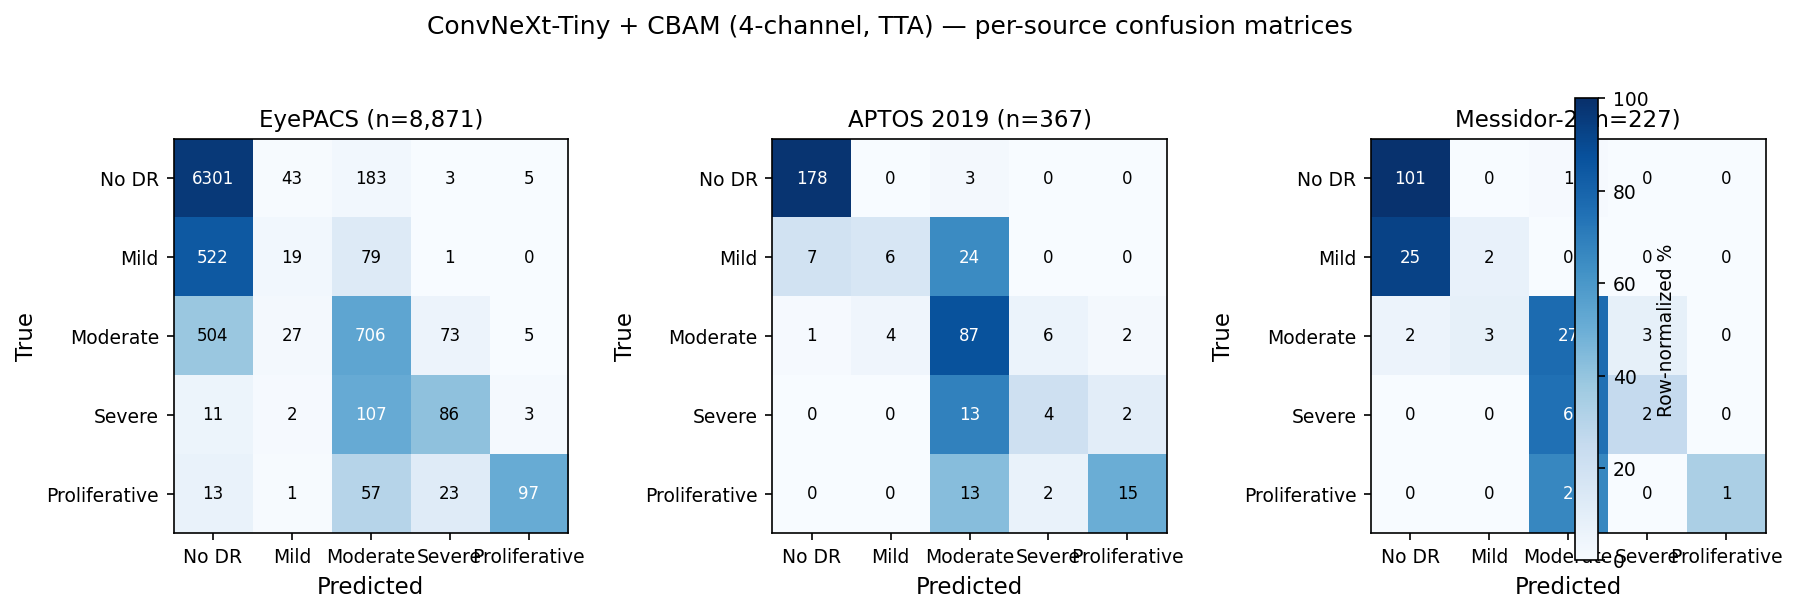
\includegraphics[width=0.95\textwidth]{figures/fig2_confusion_matrices.png}
\caption{Per-source confusion matrices for ConvNeXt-Tiny + CBAM (4-channel, TTA on). Cell values are raw counts; color encodes row-normalized percentage.}
\label{fig:cm}
\end{figure}

\subsection{Comparison to legacy 3-phase RGB baseline}

Table~\ref{tab:vs-legacy} compares against our legacy 3-phase RGB-only ConvNeXt-Tiny baseline (EyePACS pretraining $\to$ APTOS fine-tuning). The multi-domain 4-channel pipeline is strictly better on both target datasets.

\begin{table}[t]
\centering
\caption{Multi-domain 4-channel vs.\ legacy 3-phase RGB-only.}
\label{tab:vs-legacy}
\begin{tabular}{lrrr}
\toprule
Eval set & Legacy QWK (no TTA) & Multi-dom 4-ch QWK (TTA) & $\Delta$ \\
\midrule
APTOS 2019  & 0.8697 & \textbf{0.8848} & $+0.015$ \\
Messidor-2  & 0.6146 (zero-shot) & \textbf{0.8376} (in-distribution) & $+0.223$ \\
\bottomrule
\end{tabular}
\end{table}

\subsection{Architecture comparison}

We trained three architectures through the identical multi-domain 4-channel pipeline (Figure~\ref{fig:qwk-bars}):
\begin{itemize}
  \item \textbf{ConvNeXt-Tiny + CBAM} (384$\times$384): our headline model.
  \item \textbf{SwinV2-Tiny + CBAM} (256$\times$256): the smaller-resolution ablation.
  \item \textbf{ConvNeXt+Swin ensemble}: probability-averaged across the two.
\end{itemize}

\begin{figure}[t]
\centering
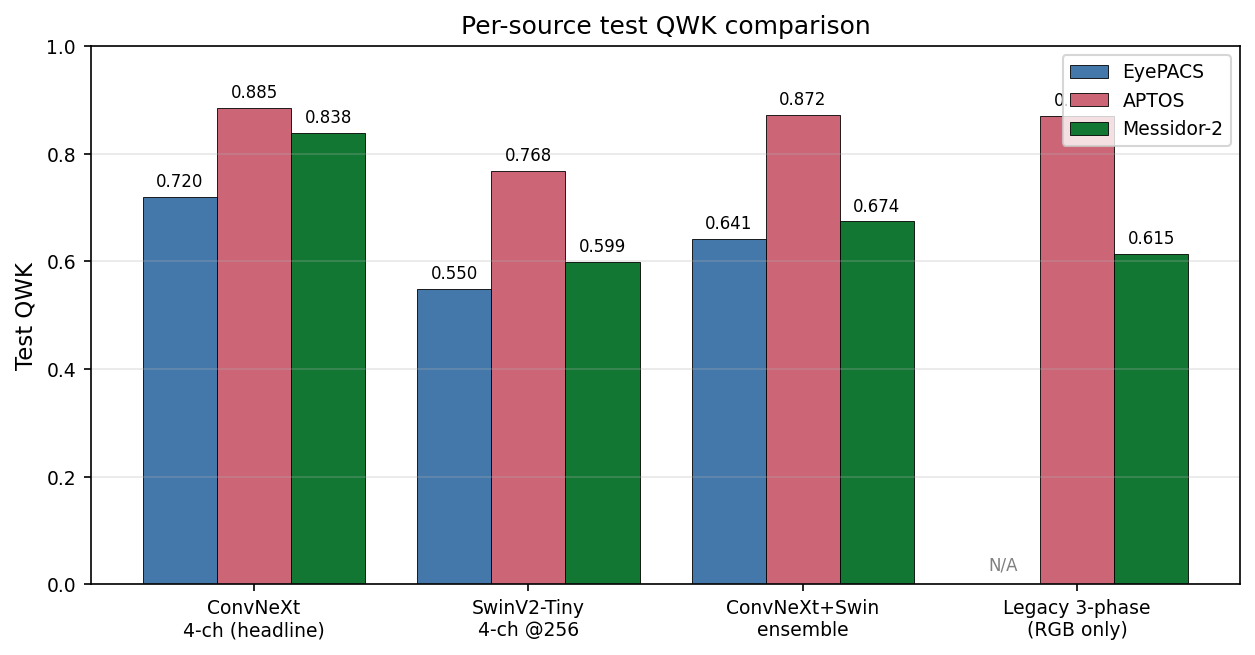
\includegraphics[width=0.95\textwidth]{figures/fig3_qwk_comparison.png}
\caption{Per-source test QWK across three architectures and the legacy baseline. The ConvNeXt+Swin ensemble underperforms the ConvNeXt-only model at every site, indicating that Swin's weaker per-class accuracy at 256$\times$256 drags down the averaged probabilities.}
\label{fig:qwk-bars}
\end{figure}

SwinV2-Tiny at 256$\times$256 loses approximately $0.15$ QWK per site relative to ConvNeXt at 384$\times$384, consistent with the $\sim$3$\times$ smaller spatial pixel budget degrading fine-grained lesion localization. The naive ensemble \emph{hurts} on every site, because Swin's lower-quality probabilities pull down the average.

\subsection{Negative result: EfficientNetV2-S training fails}

Two EfficientNetV2-S training attempts failed with catastrophic val-loss explosion at the start of Phase 2 (full fine-tune), despite reductions in learning rate from $1.22 \times 10^{-4}$ to $2 \times 10^{-5}$ (Figure~\ref{fig:effnet-explosion}). Diagnostic analysis reveals that the saved Phase-1 checkpoint produces reasonable logits in train mode (BatchNorm using batch statistics, range $[-3, +3]$) but extreme logits in eval mode (BatchNorm using running statistics, range $[-68{,}000, +367{,}000]$, standard deviation $81{,}000$). The CORN loss with binary-cross-entropy saturates at these magnitudes, yielding val loss $> 32{,}000$ on the very first Phase-2 epoch. The cause appears to be BatchNorm running-statistics divergence at the frozen-to-unfrozen boundary; resetting running statistics to $(0, 1)$ at the transition (our attempted fix) does not help. The ConvNeXt-Tiny baseline is unaffected because it uses LayerNorm, which has no running statistics.

\begin{figure}[t]
\centering
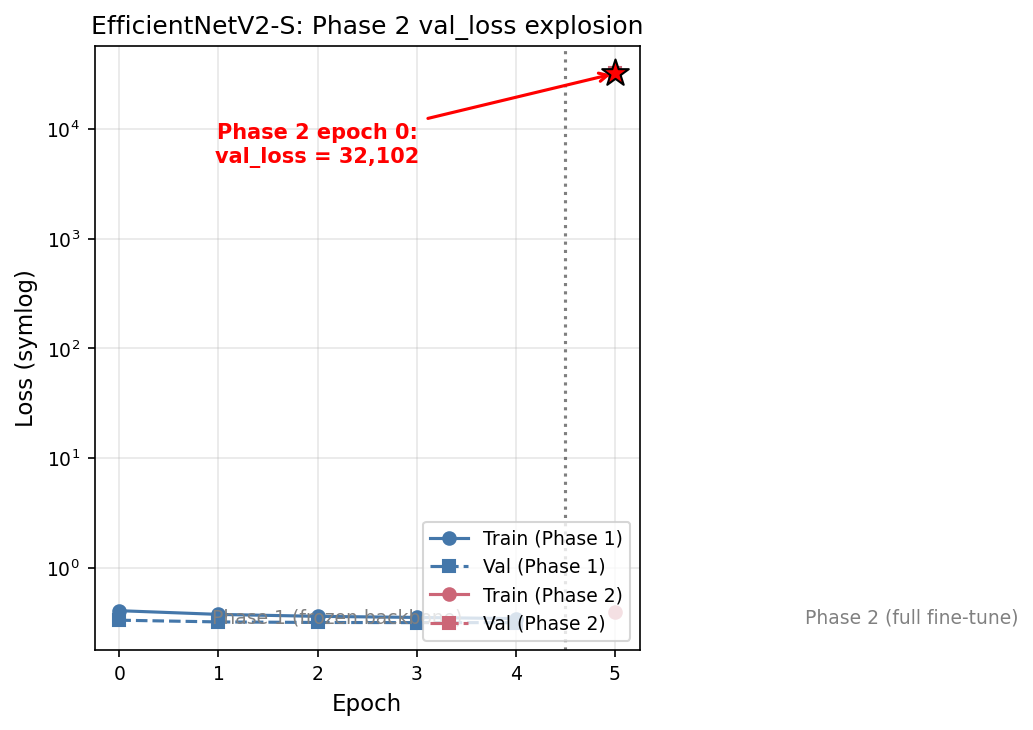
\includegraphics[width=0.95\textwidth]{figures/fig4_effnetv2_loss_explosion.png}
\caption{EfficientNetV2-S training trajectory. Phase 1 val loss $\approx 0.5$ is healthy. Phase 2 epoch 0 val loss jumps to $32{,}102$ (red star), with QWK collapsing to $0.019$.}
\label{fig:effnet-explosion}
\end{figure}

\section{Discussion}

\subsection{Why multi-domain training helps}

Messidor-2 is the smallest source (1{,}815 images), and on the legacy 3-phase setup it was held out entirely from training: the model had to generalize zero-shot from EyePACS+APTOS to Messidor-2. This gave Messidor-2 QWK of $0.6146$. Including Messidor-2 in the training set brings in-distribution Messidor-2 QWK to $0.8376$, a $+0.22$ absolute gain that is the largest single source of improvement in the project.

The cost is mild degradation on APTOS (the original legacy model was APTOS-fine-tuned specifically), but the multi-domain APTOS QWK of $0.8848$ still beats the legacy $0.8697$.

\subsection{Why the segmentation channel helps}

The 4-channel input (3 RGB + 1 vessel/lesion mask) provides the grader with explicit anatomical cues that are camera-agnostic. The U-Net was trained on DRIVE+IDRiD, neither of which is in the grading test sets, so the masks at test time are generalizing from a different domain than the segmentation training domain. Despite this, they help: the multi-domain 4-channel model is strictly better than the RGB-only legacy model on APTOS and dramatically better on Messidor-2.

\subsection{Why SwinV2-Tiny underperforms}

SwinV2-Tiny's native input resolution is 256$\times$256. We resize our 384$\times$384 preprocessed images down to 256$\times$256 at training and inference. The 384$\times$384 ConvNeXt has $\sim$3$\times$ more pixels per image, which matters disproportionately for fine-grained ordinal boundaries (mild vs.\ no DR, moderate vs.\ severe). The ensemble attempt fails because Swin's lower-quality probability distributions pull the averaged probabilities toward Swin's incorrect predictions.

\subsection{Negative result discussion: EffNetV2-S}

The EfficientNetV2-S failure is instructive. Two attempts with very different learning rates (a 60$\times$ range) both fail at the same point: the unfreeze boundary. Diagnostic eval-mode inspection of the saved checkpoint shows extreme logit magnitudes consistent with BatchNorm running-statistics not tracking the activation distribution. We document this in detail in the project repository at \texttt{saved/logs/effnetv2\_root\_cause.md} but did not find a fix within the project's time budget.

\section{Conclusions}

GradeEye is a competitive diabetic retinopathy grading pipeline that improves over our legacy three-phase baseline on every test site we evaluated. The headline result, ConvNeXt-Tiny + CBAM with a four-channel input and multi-domain training, achieves $0.7196$ QWK on EyePACS test, $0.8848$ on APTOS 2019, and $0.8376$ on Messidor-2 (in-distribution). Multi-domain training and the anatomical segmentation channel are the two largest contributors; CORN ordinal regression provides structurally rank-consistent predictions at inference time.

Two negative results are reported for completeness: EfficientNetV2-S failed to converge due to a BatchNorm running-statistics issue at the phase transition, and SwinV2-Tiny at 256$\times$256 underperformed ConvNeXt at 384$\times$384 on every test site. Future work would focus on diagnosing and fixing the EffNetV2-S issue (to provide a robust second architecture), training at the original SwinV2 resolution of 384$\times$384 if a compatible pretrained checkpoint becomes available, and exploring whether the segmentation mask can be made richer (e.g., a 5-channel output for vessel plus each lesion type rather than a single union).

\section*{Reproducibility}

The codebase is structured as:
\begin{itemize}
  \item \texttt{configs/} --- YAML run configurations.
  \item \texttt{src/} --- preprocessing, datasets, models (ConvNeXt / EffNetV2-S / Swin / U-Net), losses (CORN), training (EMA, optimizer, trainer), evaluation.
  \item \texttt{scripts/} --- CLI drivers for preprocessing, segmentation, training, evaluation, ensemble evaluation, and figure generation.
  \item \texttt{data/processed/segmentation\_combined/} --- the 93{,}111 precomputed 384$\times$384 segmentation masks.
\end{itemize}

Training and evaluation require approximately 5 hours per ConvNeXt-Tiny run on a single GPU. The exact checkpoints, logs, and split CSVs are preserved in the project repository.

\end{document}